\documentclass[final]{beamer}

\usepackage[scale=1.24]{beamerposter} % Use the beamerposter package for laying out the poster
\usepackage{tikz}

\usetheme{confposter}

\setbeamercolor{block title}{fg=ngreen,bg=white} % Colors of the block titles
\setbeamercolor{block body}{fg=black,bg=white} % Colors of the body of blocks
\setbeamercolor{block alerted title}{fg=white,bg=dblue!70} % Colors of the highlighted block titles
\setbeamercolor{block alerted body}{fg=black,bg=dblue!10} % Colors of the body of highlighted blocks
\addtobeamertemplate{block begin}{\setlength\abovedisplayskip{0pt}}


\newcommand{\redc}[2][red,fill=red]{\tikz[baseline=-0.5ex]\draw[#1,radius=#2] (0,0) circle ;}%
\newcommand{\bluec}[2][blue,fill=blue]{\tikz[baseline=-0.5ex]\draw[#1,radius=#2] (0,0) circle ;}%

%-----------------------------------------------------------
% Define the column widths and overall poster size
% To set effective sepwid, onecolwid and twocolwid values, first choose how many columns you want and how much separation you want between columns
% In this template, the separation width chosen is 0.024 of the paper width and a 4-column layout
% onecolwid should therefore be (1-(# of columns+1)*sepwid)/# of columns e.g. (1-(4+1)*0.024)/4 = 0.22
% Set twocolwid to be (2*onecolwid)+sepwid = 0.464
% Set threecolwid to be (3*onecolwid)+2*sepwid = 0.708

\newlength{\sepwid}
\newlength{\onecolwid}
\newlength{\twocolwid}
\newlength{\threecolwid}
\newlength{\figwid}
\setlength{\paperwidth}{48in} % A0 width: 46.8in
\setlength{\paperheight}{36in} % A0 height: 33.1in
% \setlength{\sepwid}{0.024\paperwidth} % Separation width (white space) between columns
\setlength{\sepwid}{1ex} % Separation width (white space) between columns
% \setlength{\onecolwid}{0.32\paperwidth} % Width of one column
\setlength{\onecolwid}{0.32\paperwidth} % Width of one column
\setlength{\twocolwid}{0.464\paperwidth} % Width of two columns
\setlength{\threecolwid}{0.708\paperwidth} % Width of three columns
\setlength{\topmargin}{-0.5in} % Reduce the top margin size
\setlength{\figwid}{.55\onecolwid}
%-----------------------------------------------------------

\usepackage{graphicx}  % Required for including images
\usepackage{eso-pic}
\usepackage{booktabs} % Top and bottom rules for tables




%----------------------------------------------------------------------------------------
%	TITLE SECTION
%----------------------------------------------------------------------------------------

\title{Simulation and Theory of Bacterial Transformation} % Poster title

\author{JD Russo, Jiajia Dong} % Author(s)

\institute{Department of Physics and Astronomy, Bucknell University} % Institution(s)


\begin{document}

% \addtobeamertemplate{block end}{}{\vspace*{1ex}} % White space under blocks
% \addtobeamertemplate{block alerted end}{}{\vspace*{1ex}} % White space under highlighted (alert) blocks

\setlength{\belowcaptionskip}{2ex} % White space under figures
\setlength\belowdisplayshortskip{2ex} % White space under equations

\newcommand\AtPagemyUpperLeft[1]{\AtPageLowerLeft{%
% \put(\LenToUnit{0.89\paperwidth},\LenToUnit{0.92\paperheight}){#1}}}
\put(\LenToUnit{0.83\paperwidth},\LenToUnit{0.005\paperheight}){#1}}}
\AddToShipoutPictureFG{
  \AtPagemyUpperLeft{{
\includegraphics[width=12cm,keepaspectratio]{bucknell.pdf}}}
}%


\begin{frame}[t] % The whole poster is enclosed in one beamer frame

\begin{block}

\begin{columns}[t] % The whole poster consists of three major columns, the second of which is split into two columns twice - the [t] option aligns each column's content to the top
\begin{column}{4ex}\end{column} % Empty spacer column

% ------------------------- First column -------------------------
\begin{column}{.85\onecolwid}

  %-------------
  %	Motivation
  %-------------
  \begin{alertblock}{Introduction}
  % \begin{itemize}
  %   \item Ubiquitous threat of antibiotic resistant bacteria
  %   \item Investigate effect of different cellular transformation rates on antibiotic
  %   resistant bacterial population growth
  % \end{itemize}
  The threat of antibiotic resistant bacteria is becoming more ubiquitous, even
  among well-controlled diseases such as tuberculosis. Main mechanisms
  for the emergence of antibiotic resistance include conjugation and transformation.
  We focus on the effect of transformation.

  \quad\quad We use a combined approach of Kinetic Monte Carlo simulation and
  mathematical
  modeling to explore interplay among \textbf{growth} ($b$), \textbf{death} ($\delta$), \textbf{transformation} ($\alpha$), and \textbf{plasmid availability} ($P$).
  Numerically modelling the populations with their
  associated differential equations provides information about long-term
  population behavior, while K.M.C. simulation provides information about dynamics.

  \quad\quad We study differential growth and transformation to
  determine what most affects whether the susceptible or resistant population
  dominates.
  \end{alertblock}
\end{column}

% ----------------------------------------------------------------
\begin{column}{10\sepwid}\end{column} % Empty spacer column

% ------------------------- Second column -------------------------
\begin{column}{.9\onecolwid}
  %-------------
  %	INTRODUCTION
  %-------------
  \begin{alertblock}{Biological Background}
    % \begin{itemize}
    %   \item Plasmids
    %   \item Fitness cost
    %   \item Transformation
    % \end{itemize}
    \textbf{Plasmids} are small independently replicating genetic materials,
    often including DNA segments encoding antibiotic resistance.

    \quad\quad Through \textbf{transformation} a cell can incorporate
    a physical plasmid and translate the encoded genes. However, this often
    comes with a small fitness cost to the carrying cell, typically manifesting
    as a longer doubling time.

    \vspace{2ex}

    \begin{center}
      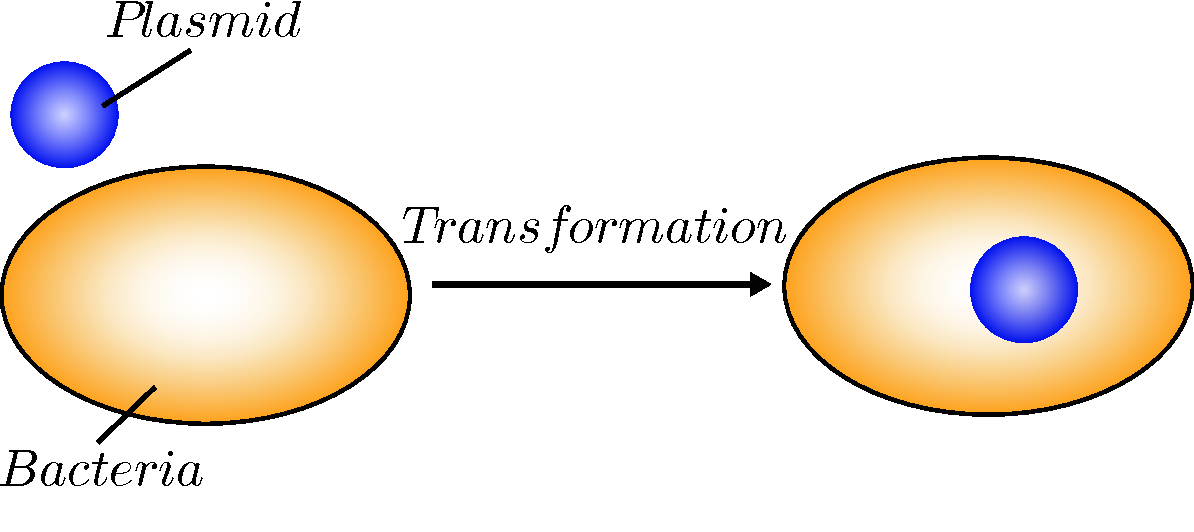
\includegraphics[width=.8\figwid]{../dev/graphics/poster/transformation.pdf}
    \end{center}
  \end{alertblock}
\end{column}

\begin{column}{10\sepwid}\end{column} % Empty spacer column

% ------------------------- Third column -------------------------
\begin{column}{1.2\onecolwid}
  %-------------
  %	Motivation
  %-------------
  \begin{alertblock}{Simulation Methods}
    % \begin{itemize}
    %   \item Combined approach of Kinetic Monte Carlo simulation and numerical modeling
    %   \item Gillespie algorithm
    %   \item Well-mixed population
    %   \item Carrying capacity
    %   \item Constant, Linear, Recycled $\alpha$
    %   \item Symmetric division
    %   \item Realtime conversion
    % \end{itemize}
    We examine the \textbf{susceptible} ($S$) and \textbf{resistant} ($R$) populations
    with a combined approach of numerical modeling methods and Kinetic Monte
    Carlo simulation.

    \quad\quad Kinetic Monte Carlo simulation allows us to
    capture information about the dynamics of the populations. We implement the
    Gillespie algorithm, which consists of the following steps:
    \begin{center}
    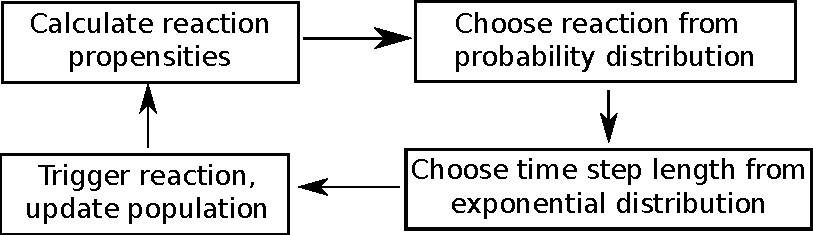
\includegraphics[width=\figwid]{../dev/graphics/poster/gillespie.pdf}
    \end{center}

    \quad\quad We assume a well-mixed environment, a fixed carrying capacity $K$, and
    that reproduction occurs symmetrically for both $S$ and $R$. This does not conserve total
    plasmid number.

    \vspace{1ex}
  \end{alertblock}
\end{column}
% ----------------------------------------------------------------
% \begin{column}{\sepwid}\end{column} % Empty spacer column
\end{columns} % End of all the columns in the poster
\end{block}


\begin{block}

\begin{columns}[t]
% \begin{column}{\sepwid}\end{column} % Empty spacer column

% ------------------------- First column -------------------------
\begin{column}{\onecolwid}

  \setbeamercolor{block title}{fg=black,bg=white} % Colors of the block titles
  \begin{block}{Constant $\alpha$}
  \setbeamercolor{block title}{fg=ngreen,bg=white} % Colors of the block titles
  \begin{center}
    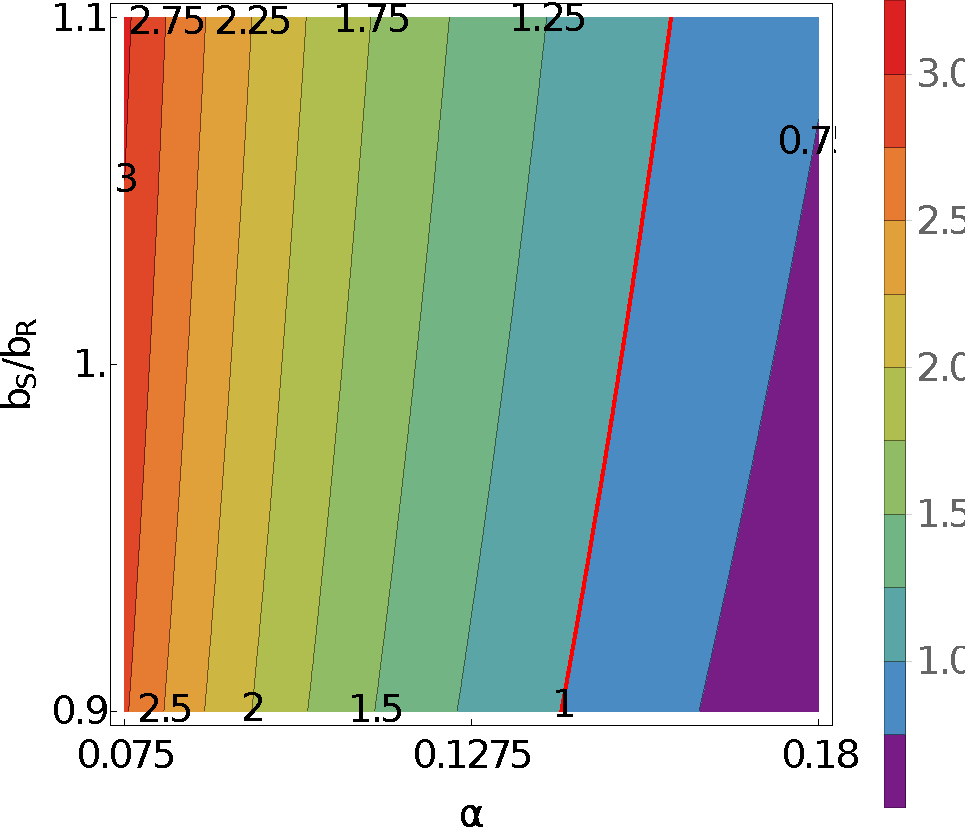
\includegraphics[width=\figwid]{../dev/graphics/poster/const_contour.pdf}
    \vspace{1.5ex}

%------------------------- Population plot and parameter table ---------------
      \begin{minipage}[h]{0.6\onecolwid}
      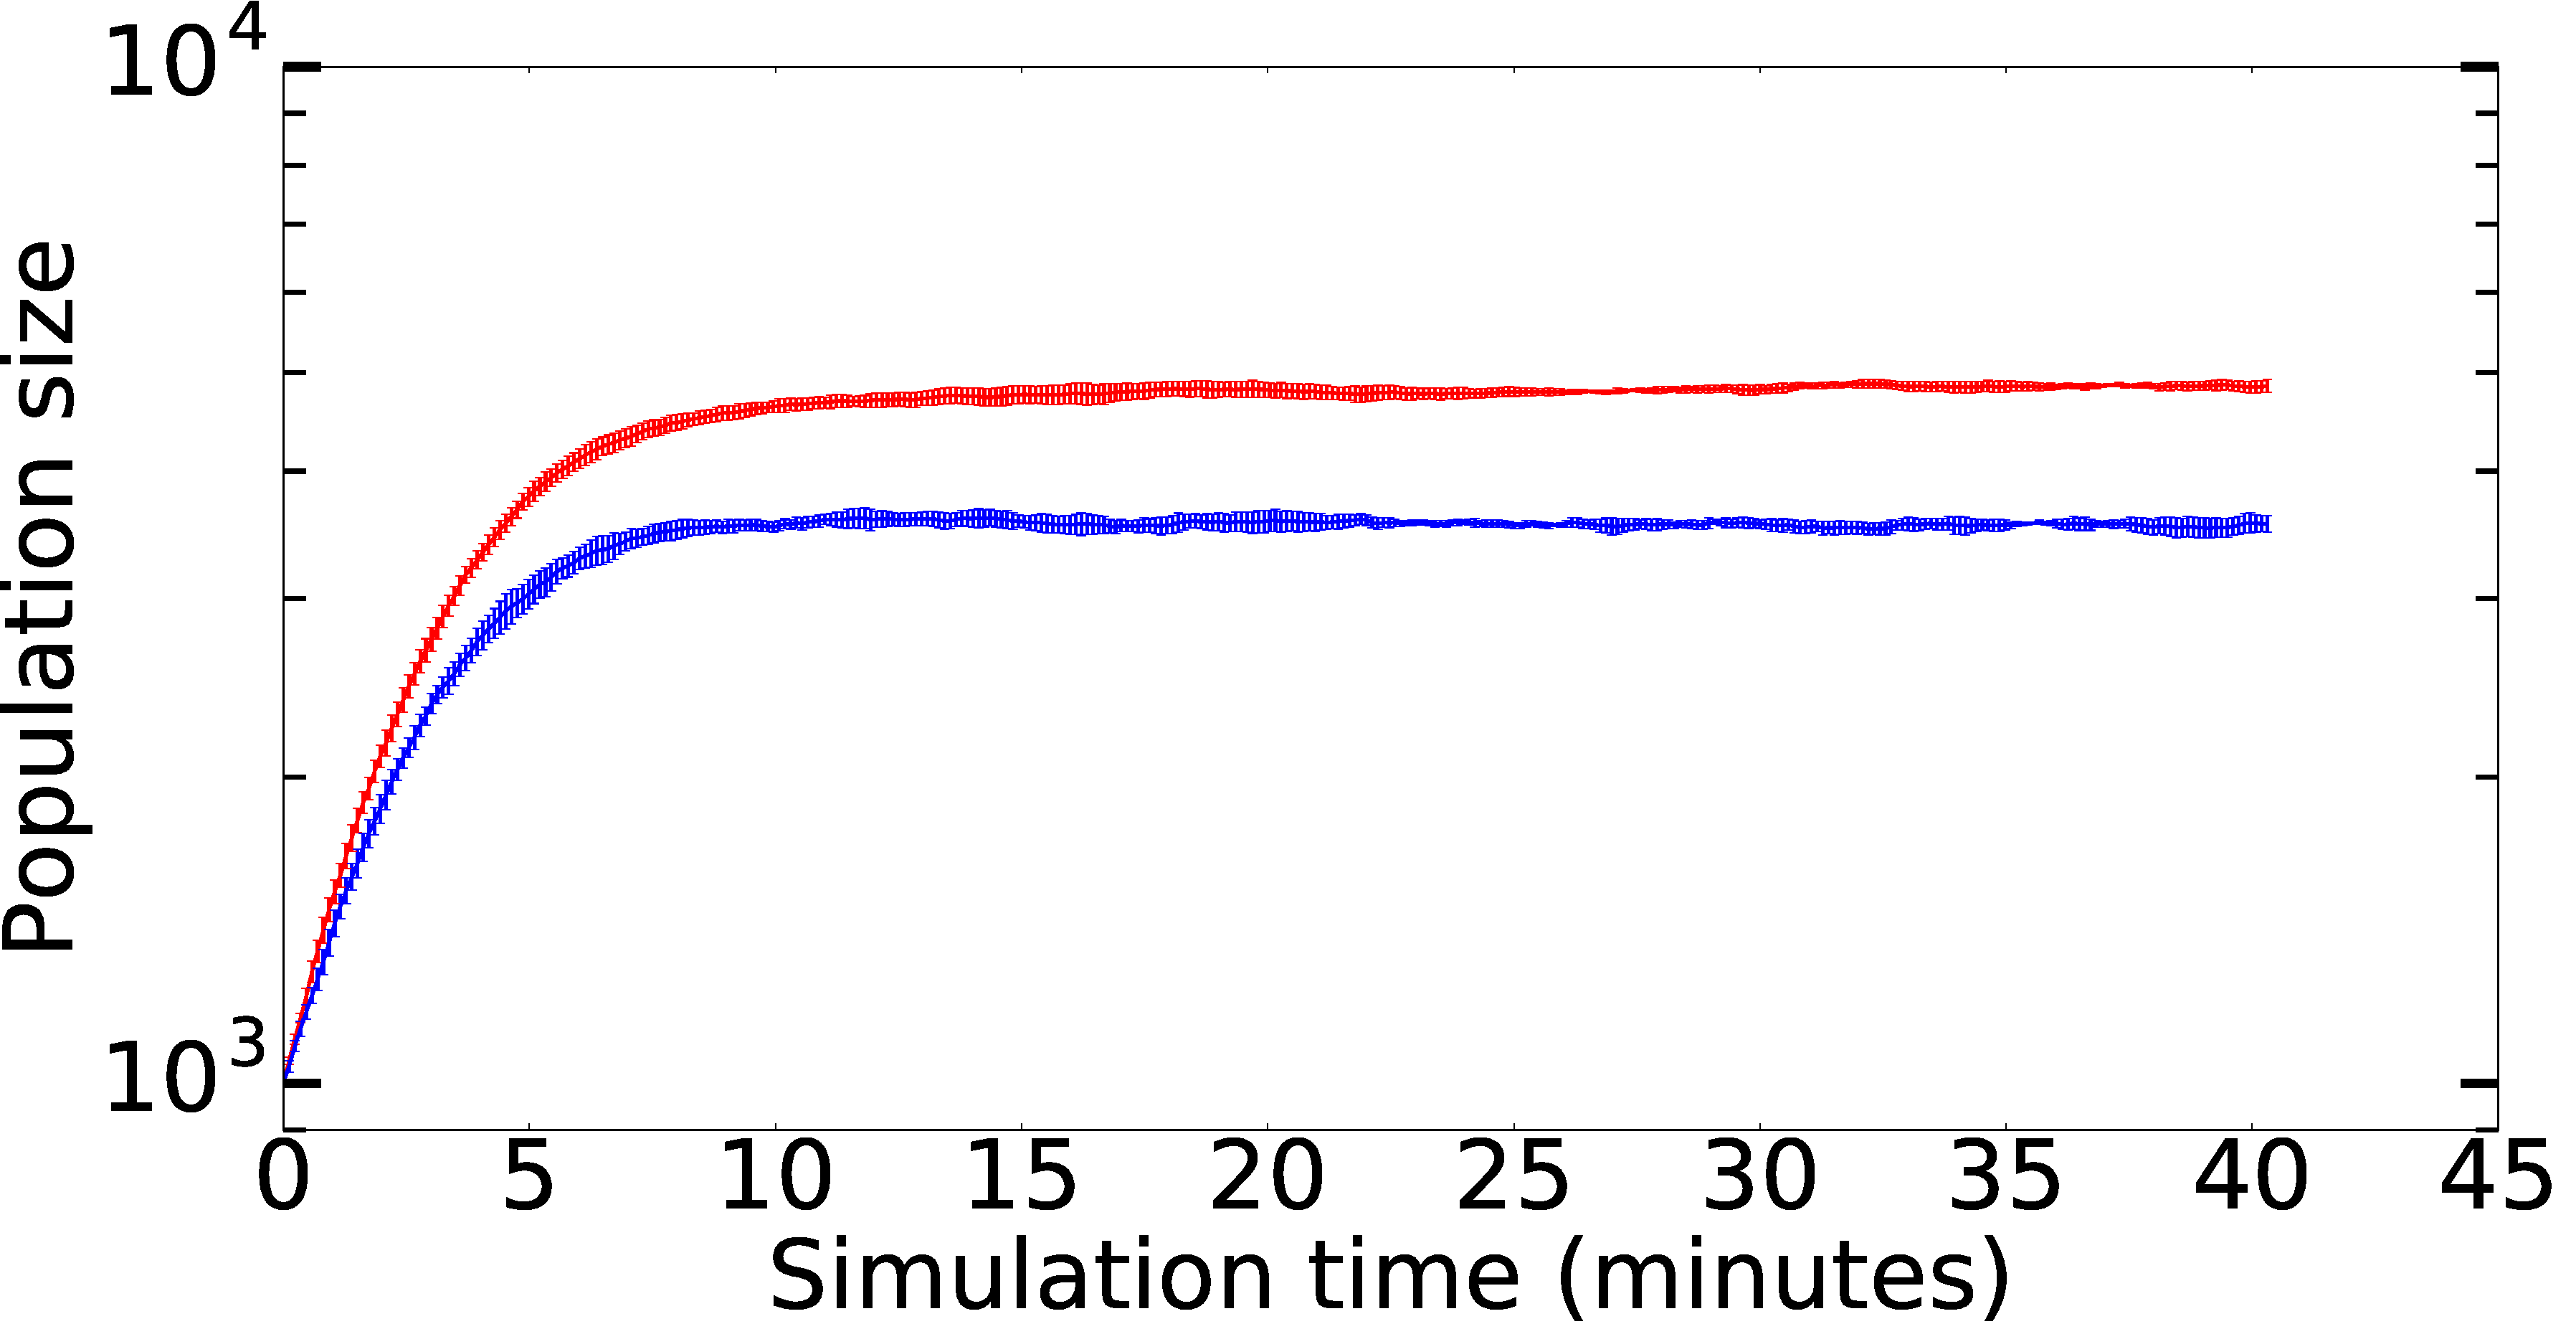
\includegraphics[width=.9\figwid]{../dev/graphics/poster/const_pop.pdf}
    \end{minipage}%
    \begin{minipage}[h]{.3\onecolwid}
      \vfill \textbf{Parameters} \vspace{3mm}\\
      \begin{tabular}{l  r  c|c  l  r}
        \toprule
        $\alpha$ & .13 & \quad & \quad &
          $\frac{b_S}{b_R}$ & 1.07 \\
        $S_0$ & $10^3$ & \quad & \quad &
          $R_0$ & $10^3$ \\
        $P_0$ & $10^4$ & \quad & \quad &
          $K$ & $10^4$ \\
          \bottomrule
      \end{tabular}\\\vspace{1ex}

      \redc{5pt}  Susceptible\\
      \bluec{5pt}  Resistant
    \end{minipage}
%-----------------------------------------------------------------------------
  \end{center}
  \hrule height 3pt
  \begin{columns}[t]
    \begin{column}{.2\onecolwid}
      \begin{center}
        Reactions
      \end{center}
      \begin{align*}
        S & \stackrel{b_S}{\rightarrow} 2S \\
        S & \stackrel{\alpha}{\rightarrow}  R \\
        R & \stackrel{b_R}{\rightarrow} 2R \\
        R & \stackrel{\delta}{\rightarrow} \varnothing
      \end{align*}
    \end{column}
      \vrule
    \begin{column}{.5\onecolwid}
      \begin{center}
        Equations
      \end{center}

      \begin{align*}
        \frac{dS}{dt}& = b_S \left(1 - \frac{S + R}{K}\right)S - \alpha S \\[0.5ex]
        \frac{dR}{dt}& = b_R \left(1 - \frac{S + R}{K}\right)R + \alpha S - \delta R
      \end{align*}

      \vspace{2.9\baselineskip}
      \vspace{1ex}
    \end{column}
  \end{columns}
  \hrule height 3pt
  \end{block}
\end{column}

% ----------------------------------------------------------------
\vrule width 5pt
\begin{column}{\sepwid}\end{column} % Empty spacer column

% ------------------------- Second column -------------------------
\begin{column}{.9\onecolwid}

  \setbeamercolor{block title}{fg=BurntOrange,bg=white} % Colors of the block titles
  \begin{block}{Linear $\alpha$}
  \setbeamercolor{block title}{fg=ngreen,bg=white} % Colors of the block titles
    \begin{center}
      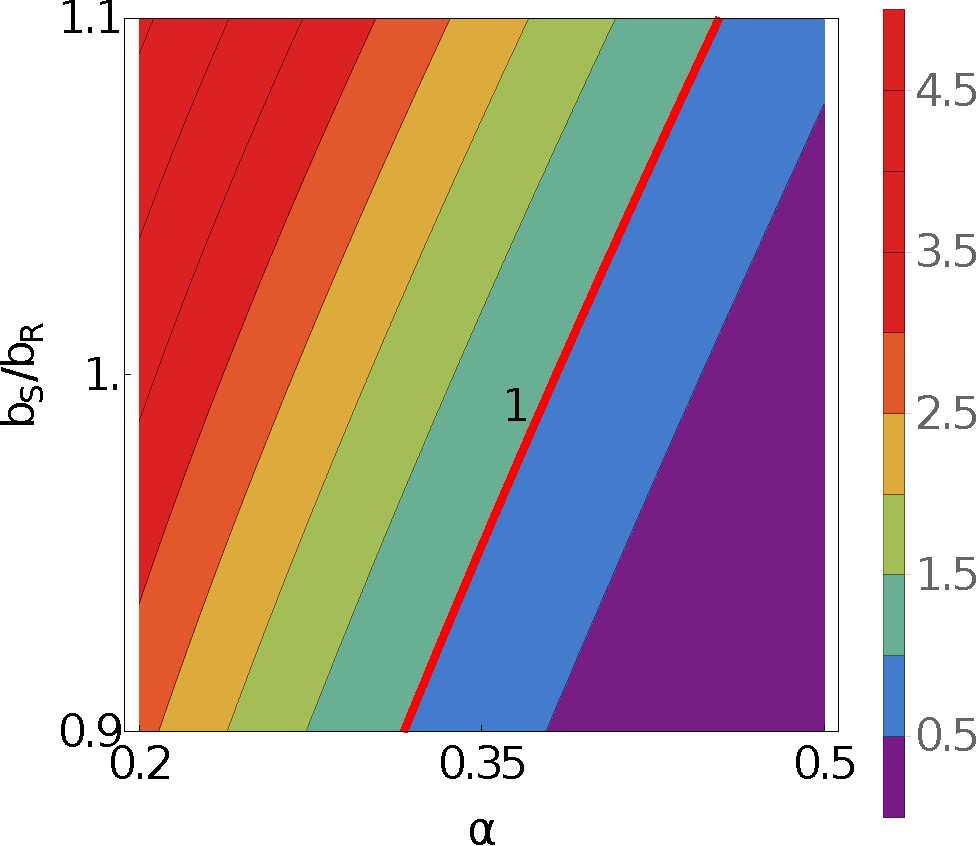
\includegraphics[width=\figwid]{../dev/graphics/poster/linear_contour.pdf}
      \vspace{1.5ex}

%------------------------- Population plot and parameter table ---------------
        \begin{minipage}[h]{0.6\onecolwid}
        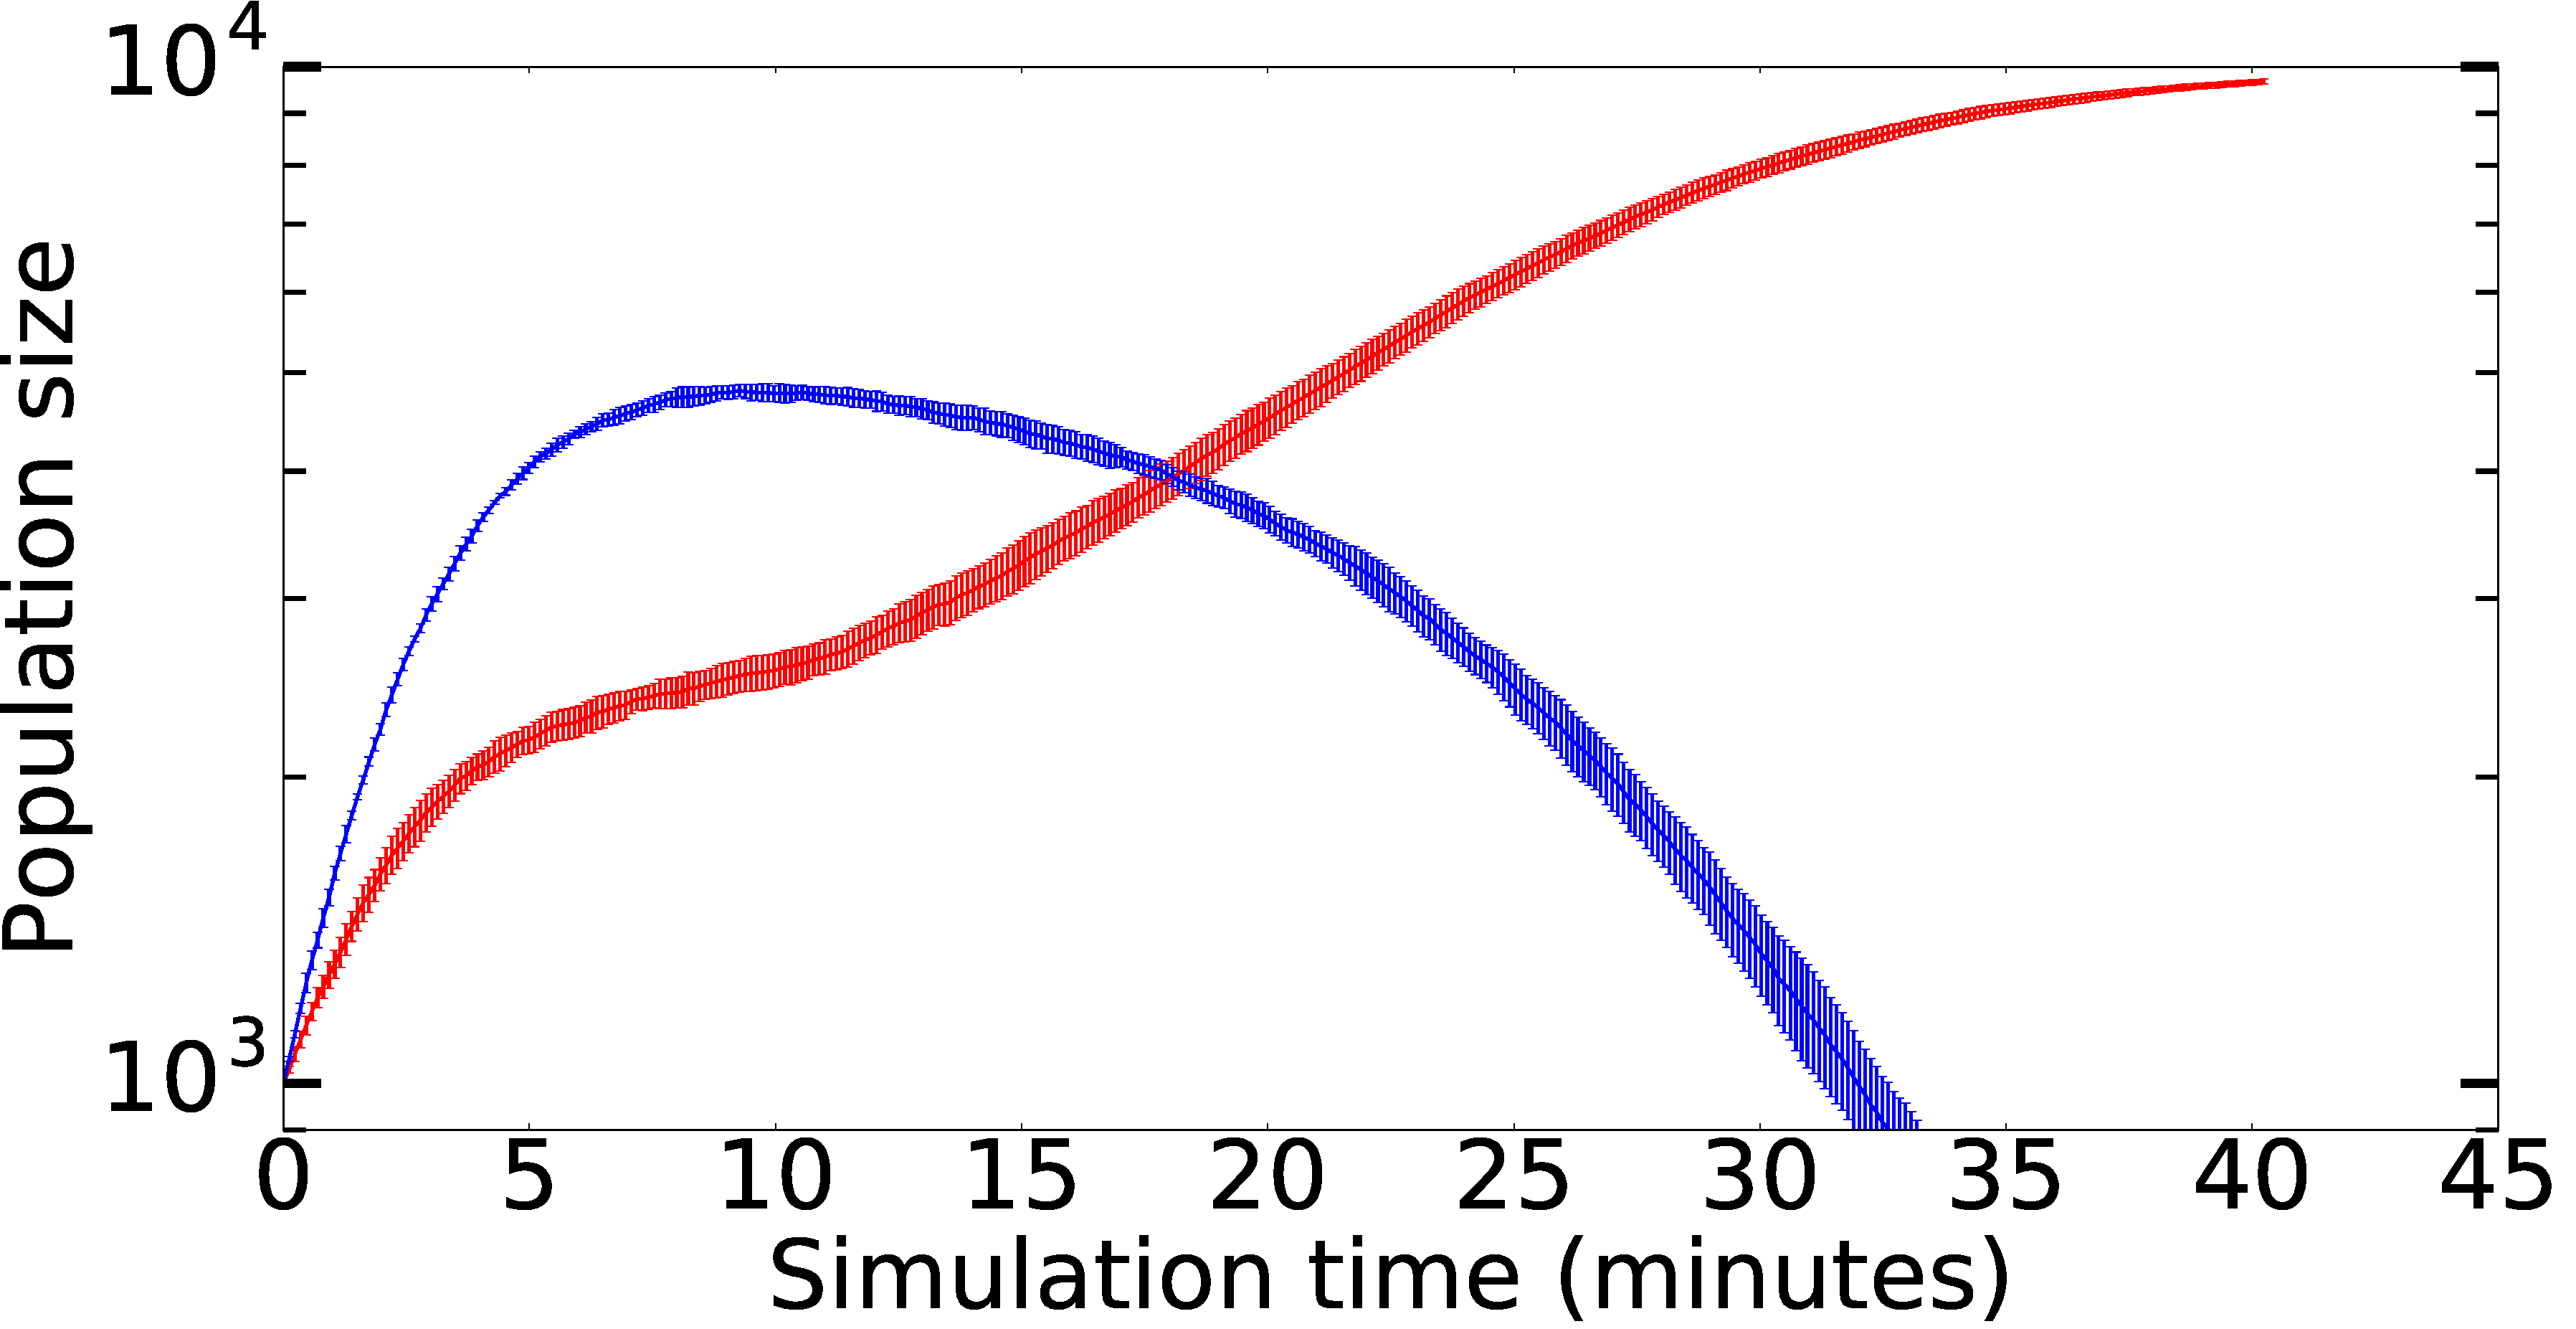
\includegraphics[width=.9\figwid]{../dev/graphics/poster/linear_pop.pdf}
      \end{minipage}%
      \begin{minipage}[h]{.3\onecolwid}
        \vfill \textbf{Parameters} \vspace{3mm}\\
        \begin{tabular}{l  r  c|c  l  r}
          \toprule
          $\alpha$ & .3 & \quad & \quad &
            $\frac{b_S}{b_R}$ & 1.07 \\
          $S_0$ & $10^3$ & \quad & \quad &
            $R_0$ & $10^3$ \\
          $P_0$ & $10^4$ & \quad & \quad &
            $K$ & $10^4$ \\
            \bottomrule
        \end{tabular}\\\vspace{1ex}

        \redc{5pt}  Susceptible\\
        \bluec{5pt}  Resistant
      \end{minipage}
%-----------------------------------------------------------------------------
    \end{center}
    \hrule height 3pt

    \begin{columns}[t]
      \begin{column}{.2\onecolwid}
        \begin{center}
          Reactions
        \end{center}
        \begin{align*}
          S & \stackrel{b_S}{\rightarrow} 2S \\
          S \color{BurntOrange}+ P\color{black} & \stackrel{\alpha}{\rightarrow}  R \\[0.8ex]
          R &\stackrel{b_R}{\rightarrow} 2R \\
          R &\stackrel{\delta}{\rightarrow} \varnothing
        \end{align*}
      \end{column}
        \vrule
      \begin{column}{.6\onecolwid}
        \begin{center}
          Equations
        \end{center}

        \begin{align*}
          \frac{dS}{dt} & = b_S \left(1 - \frac{S + R}{K}\right)S - \alpha
            \color{BurntOrange}\left( \frac{P}{P_0} \right)\color{black} S \\[0.8ex]
          \frac{dR}{dt} & = b_R \left(1 - \frac{S + R}{K}\right)R + \
            \alpha \color{BurntOrange}\left( \frac{P}{P_0} \right)\color{black} S - \delta R \\[0.8ex]
          \color{BurntOrange} \frac{dP}{dt} & \color{BurntOrange} = -\alpha \left( \frac{P}{P_0} \right) S \color{black}
        \end{align*}
        \vspace{1ex}
      \end{column}
    \end{columns}
    \hrule height 3pt
  \end{block}
\end{column}

\vrule width 5pt
\begin{column}{1.5\sepwid}\end{column} % Empty spacer column
% ------------------------- Third column -------------------------
\begin{column}{\onecolwid}

  \setbeamercolor{block title}{fg=Purple,bg=white} % Colors of the block titles
  \begin{block}{Recycled $\alpha$}
  \setbeamercolor{block title}{fg=ngreen,bg=white} % Colors of the block titles
    \begin{center}
      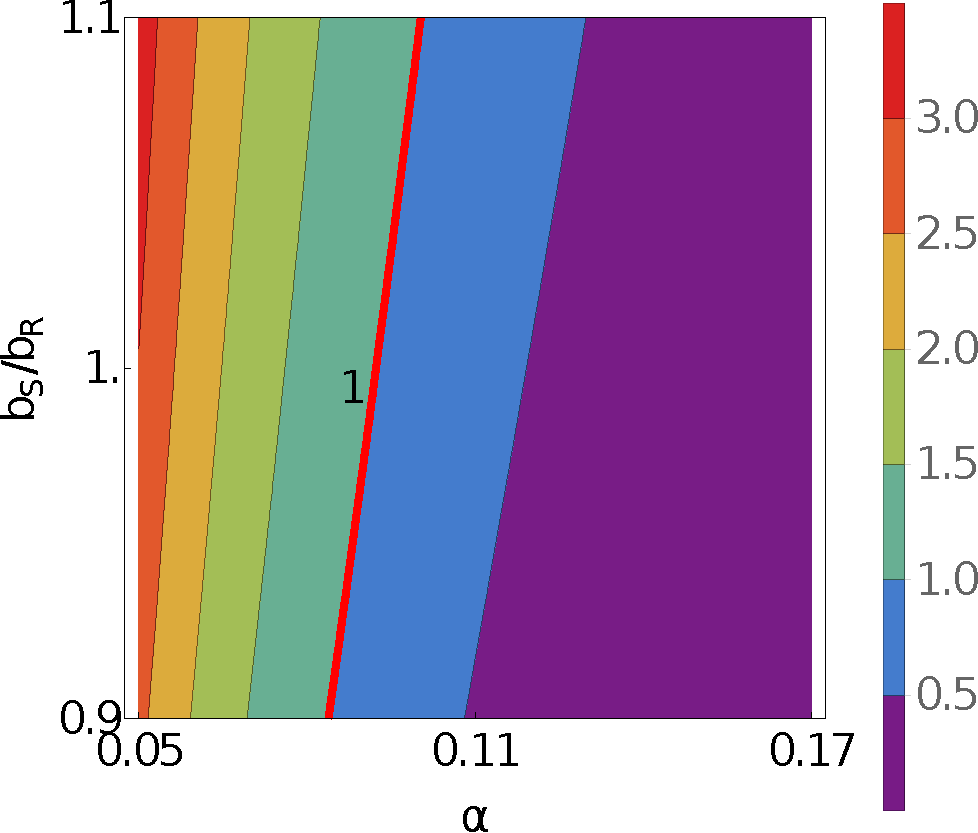
\includegraphics[width=\figwid]{../dev/graphics/poster/recycled_contour.pdf}
      \vspace{1.5ex}
%------------------------- Population plot and parameter table ---------------
        \begin{minipage}[h]{0.6\onecolwid}
        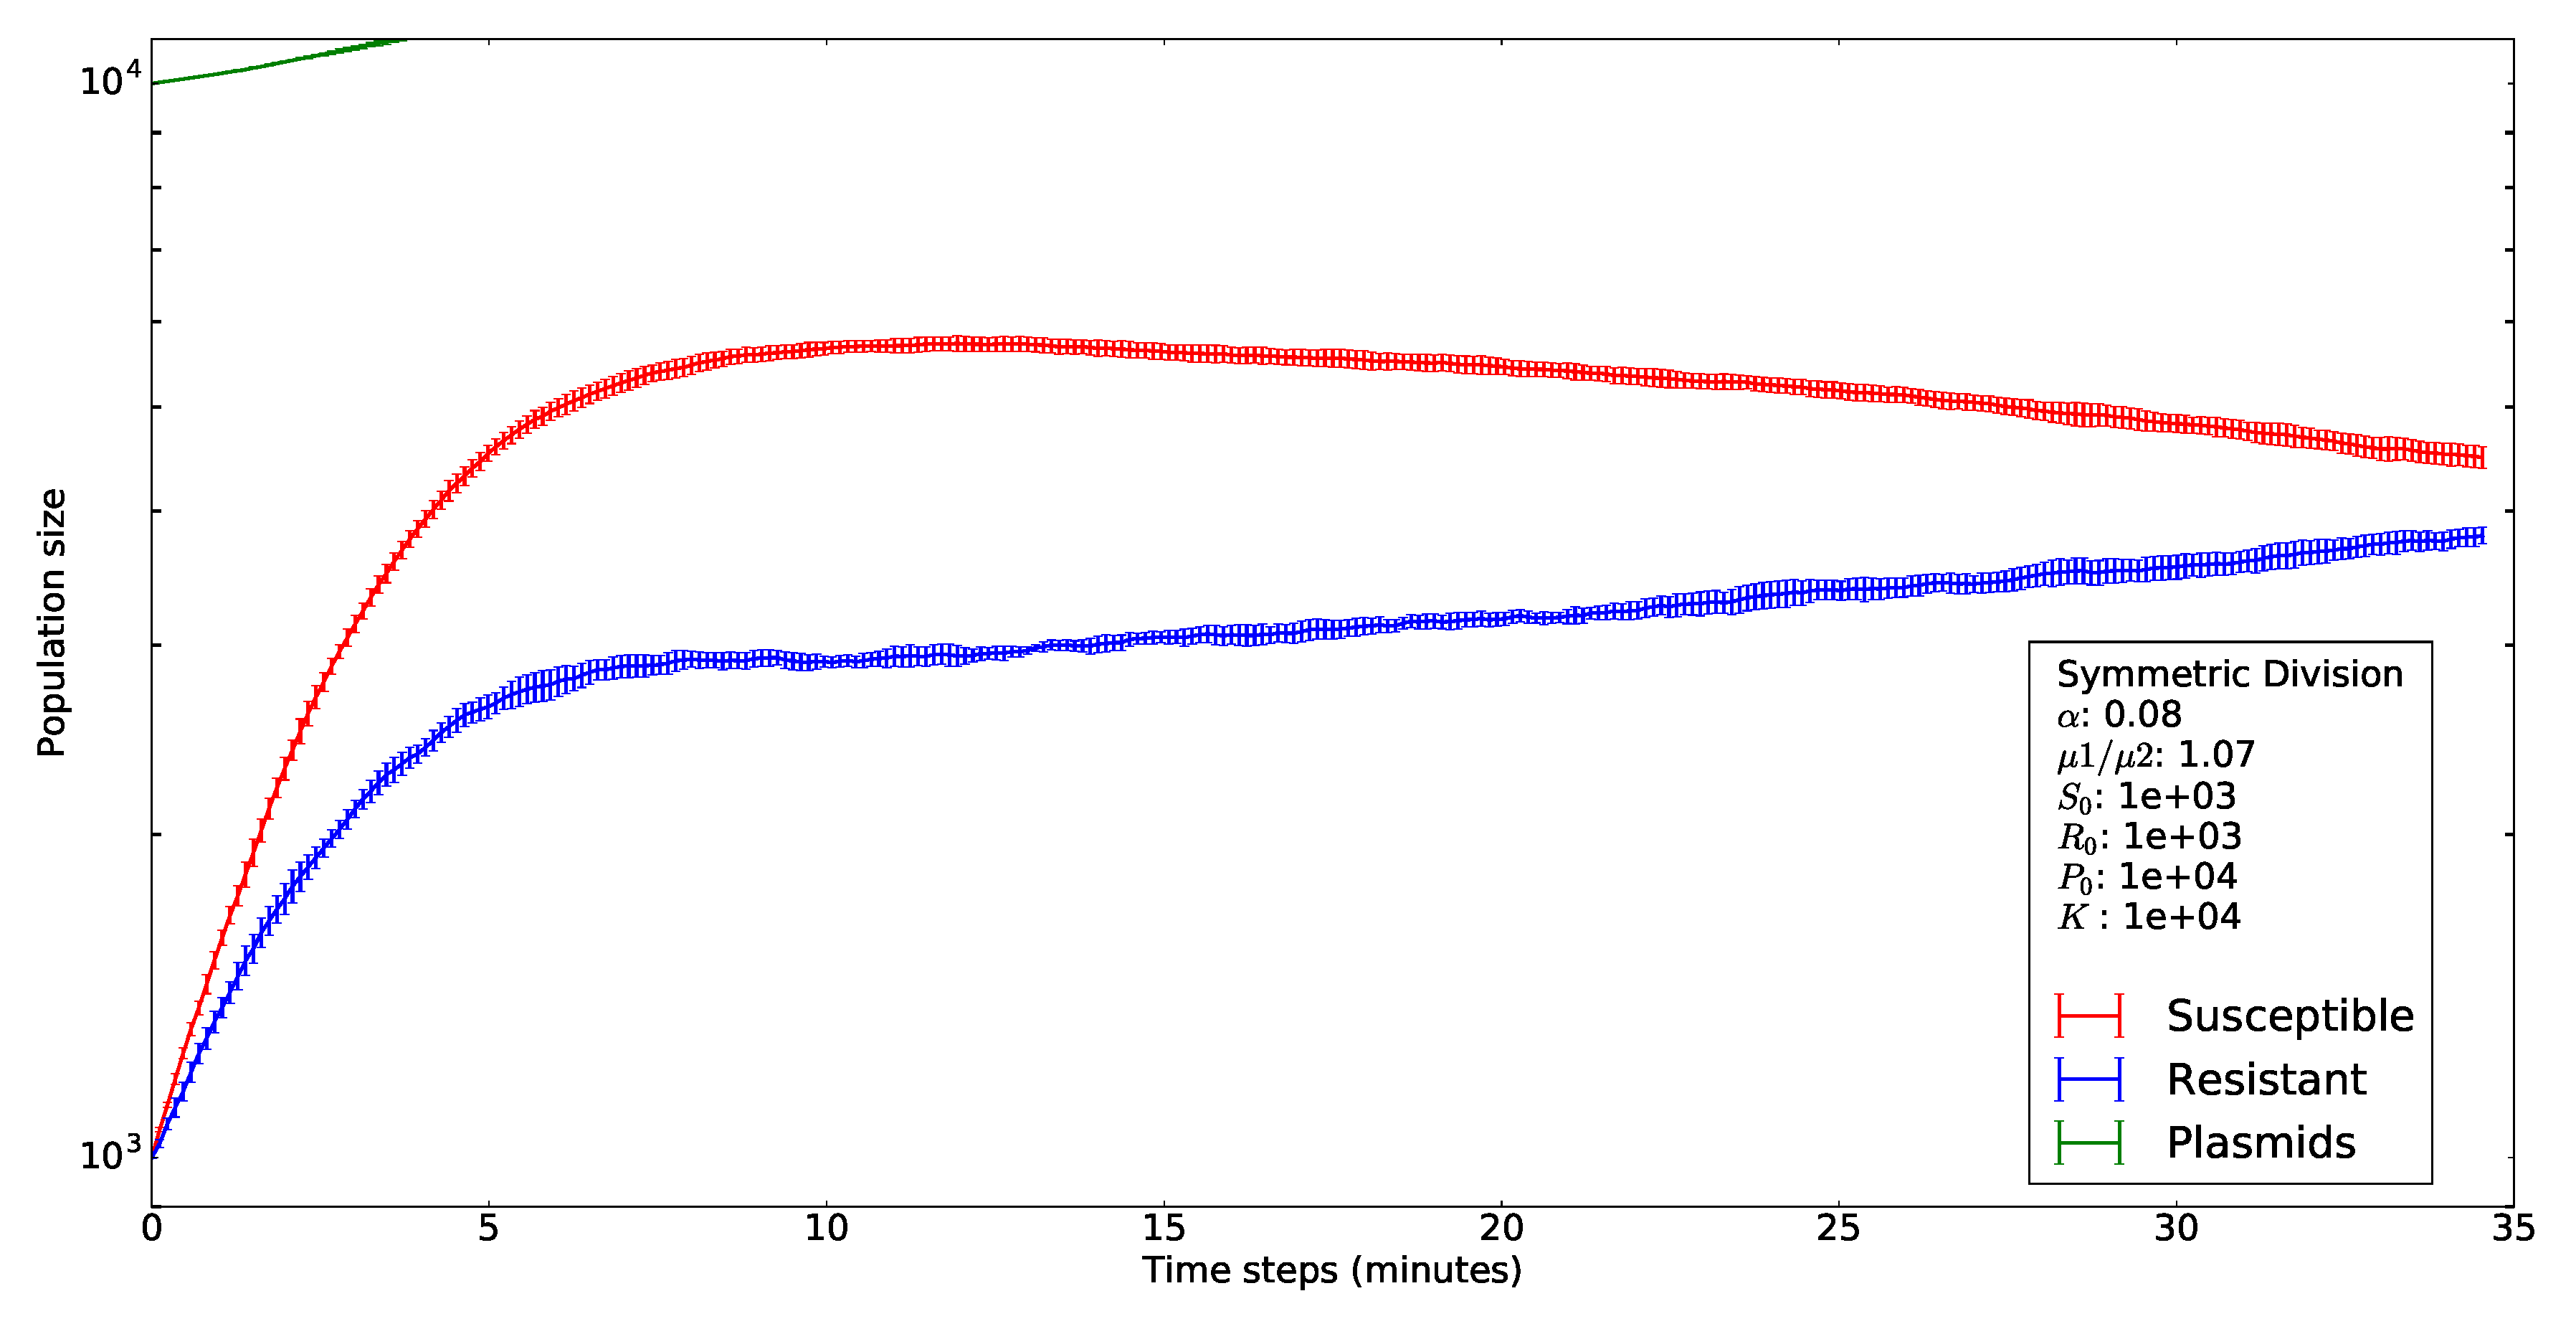
\includegraphics[width=.9\figwid]{../dev/graphics/poster/recycled_pop.pdf}
      \end{minipage}%
      \begin{minipage}[h]{.3\onecolwid}
        \vfill \textbf{Parameters} \vspace{3mm}\\
        \begin{tabular}{l  r  c|c  l  r}
          \toprule
          $\alpha$ & .13 & \quad & \quad &
            $\frac{b_S}{b_R}$ & 1.07 \\
          $S_0$ & $10^3$ & \quad & \quad &
            $R_0$ & $10^3$ \\
          $P_0$ & $10^4$ & \quad & \quad &
            $K$ & $10^4$ \\
            \bottomrule
          \end{tabular}\\\vspace{1ex}

          \redc{5pt}  Susceptible\\
          \bluec{5pt}  Resistant
      \end{minipage}
%-----------------------------------------------------------------------------

    \end{center}
    \vspace{7pt}
    \hrule height 3pt

    \begin{columns}[t]
      \begin{column}{.2\onecolwid}
        \begin{center}
          Reactions
        \end{center}
        \begin{align*}
          S & \stackrel{b_S}{\rightarrow} 2S \\
          S \color{BurntOrange}+ P\color{black} & \stackrel{\alpha}{\rightarrow}  R \\
          R & \stackrel{b_R}{\rightarrow} 2R \\
          R & \stackrel{\delta}{\rightarrow} \varnothing \color{Purple} + P \color{black}
        \end{align*}
      \end{column}
        \vrule
      \begin{column}{.75\onecolwid}
        \begin{center}
          Equations
        \end{center}

        \begin{align*}
          \frac{dS}{dt} & = b_S \left(1 - \frac{S + R}{K}\right)S - \alpha
          \color{BurntOrange} \left( \frac{P}{P_0} \right) \color{black} S +
            \color{Purple} + b_R \left(1 - \frac{S + R}{K}\right)R \color{black}  \\[0.8ex]
        \frac{dR}{dt} & =  \alpha \color{BurntOrange} \left( \frac{P}{P_0} \right) \color{black} S  - \delta R \\[0.8ex]
        \color{BurntOrange} \frac{dP}{dt} & \color{BurntOrange} = -\alpha \left( \frac{P}{P_0} \right) S \color{Purple} + \delta R \color{black}
        \end{align*}
        \vspace{1ex}
      \end{column}
    \end{columns}
    \hrule height 3pt
  \end{block}
\end{column}
% ----------------------------------------------------------------

% \begin{column}{\sepwid}\end{column} % Empty spacer column

\end{columns} % End of all the columns in the poster
\end{block}
\begin{block}

\begin{columns}[t] % The whole poster consists of three major columns, the second of which is split into two columns twice - the [t] option aligns each column's content to the top
% \begin{column}{\sepwid}\end{column} % Empty spacer column

% ------------------------- First column -------------------------
\begin{column}{1.4\onecolwid}
  %-------------
  %	Conclusions
  %-------------
  \begin{alertblock}{Conclusions}
    % \begin{itemize}
    %   \item S/R transition point depends on both rate and mechanism
    %   \item Population extinction in linear case
    % \end{itemize}
    We aimed to determine what most heavily impacts $R$ or $S$ population dominance. \\
    \quad\quad We found that the transition point where the dominant population switches
    depends heavily on both transformation rate and mechanism. In the constant case,
    long-term steady state behavior can be seen.\\
    \quad\quad Both the linear and recycled cases present examples of population
    extinction. In the linear case, the $S$ population invariably dominates,
    as plasmids are never replenished. In the recycled case, plasmid
    abundance enables the $R$ population to eventually outgrow the $S$.\\
    \quad\quad In addition, only the linear case shows significant sensitivity
    to the ratio of growth rates $b_S/b_R$.

    % \vspace{.005\baselineskip}
  \end{alertblock}
\end{column}

% ----------------------------------------------------------------
\begin{column}{\sepwid}\end{column} % Empty spacer column

% ------------------------- Second column -------------------------
\begin{column}{.9\onecolwid}
  %-------------
  %	INTRODUCTION
  %-------------
  \begin{alertblock}{Future Work}
    % \begin{itemize}
    %   \item Simulation on a lattice
    %   \item Adding antibiotics
    %   \item Asymmetric division
    % \end{itemize}
    Currently, this simulation assumes well-mixed populations of $S$, $R$, and $P$.
    A more realistic simulation could account for spatial configuration by simulating on a lattice.\\
    \quad\quad Simulating adding antibiotics to the environment could reveal situations
    where increased survivability outweighs the fitness cost of carrying a plasmid. \\
    \quad Changing $R$ division to an asymmetric scheme ($R \rightarrow R + S$) would
    yield a conserved total plasmid number.

  \end{alertblock}
\end{column}

\begin{column}{\sepwid}\end{column} % Empty spacer column

% ------------------------- Third column -------------------------
\begin{column}{.6\onecolwid}
  \begin{alertblock}{Acknowledgements}

      We would like to acknowledge the generous support provided to us by the National Science
      Foundation through the NSF grant NSF-DMR \#1248387.
      % We also thank the
      % Bucknell University Department of Physics and Astronomy.
      %
      % \vspace{5.5ex}
  \end{alertblock}
\end{column}
% ----------------------------------------------------------------
% \begin{column}{\sepwid}\end{column} % Empty spacer column
\end{columns} % End of all the columns in the poster
\end{block}
\vspace{1ex}


\end{frame} % End of the enclosing frame

\end{document}
